\documentclass[12pt]{article}
\usepackage[margin=2.5cm]{geometry}
\usepackage{enumerate}
\usepackage{amsfonts}
\usepackage{amsmath}
\usepackage{fancyhdr}
\usepackage{amsmath}
\usepackage{amssymb}
\usepackage{amsthm}
\usepackage{mdframed}
\usepackage{graphicx}
\usepackage{subcaption}
\usepackage{listings}
\usepackage{xcolor}
\usepackage[utf]{kotex}

\definecolor{codegreen}{rgb}{0,0.6,0}
\definecolor{codegray}{rgb}{0.5,0.5,0.5}
\definecolor{codepurple}{rgb}{0.58,0,0.82}
\definecolor{backcolour}{rgb}{0.95,0.95,0.92}

\lstdefinestyle{mystyle}{
    backgroundcolor=\color{backcolour},
    commentstyle=\color{codegreen},
    keywordstyle=\color{magenta},
    numberstyle=\tiny\color{codegray},
    stringstyle=\color{codepurple},
    basicstyle=\ttfamily\footnotesize,
    breakatwhitespace=false,
    breaklines=true,
    captionpos=b,
    keepspaces=true,
    numbers=left,
    numbersep=5pt,
    showspaces=false,
    showstringspaces=false,
    showtabs=false,
    tabsize=1
}

\lstset{style=mystyle}

\begin{document}
\title{CSC148 Worksheet 7 Solution}
\author{Hyungmo Gu}
\maketitle

\section*{Question 1}

\begin{itemize}
    \item Noticed that there are 11 students in total.
    \item Students should be grouped by year as closest as possible.
\end{itemize}

\bigskip

\textbf{Notes:}

\begin{itemize}
    \item 형모 해낼 뚜 있쬬!
    \item 형모 화이팅!
\end{itemize}

\section*{Question 2}
\begin{center}
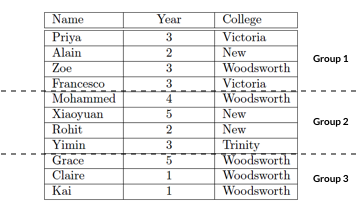
\includegraphics[width=0.7\linewidth]{images/worksheet_7_q2_solution.png}
\end{center}

\section*{Question 3}

\section*{Question 4}

\section*{Question 5}

\section*{Question 6}

\section*{Question 7}

\section*{Question 8}

\section*{Question 9}

\section*{Question 10}

\end{document}